%%%%
%% main.tex
%%
%% Copyright 2010 Jeffrey Finkelstein
%%
%% Except where otherwise noted, this work is made available under the terms of
%% the Creative Commons Attribution-ShareAlike 3.0 license,
%% http://creativecommons.org/licenses/by-sa/3.0/.
%%
%% You are free:
%%    * to Share — to copy, distribute and transmit the work
%%    * to Remix — to adapt the work
%% Under the following conditions:
%%    * Attribution — You must attribute the work in the manner specified by
%%    the author or licensor (but not in any way that suggests that they
%%    endorse you or your use of the work).
%%    * Share Alike — If you alter, transform, or build upon this work, you may
%%    distribute the resulting work only under the same, similar or a 
%%    compatible license.
%%    * For any reuse or distribution, you must make clear to others the 
%%    license terms of this work. The best way to do this is with a link to the
%%    web page http://creativecommons.org/licenses/by-sa/3.0/.
%%    * Any of the above conditions can be waived if you get permission from
%%    the copyright holder.
%%    * Nothing in this license impairs or restricts the author's moral rights.
%%%%
\documentclass{article}

% package imports
\usepackage[noend,linesnumbered,boxed]{algorithm2e} % for creating pseudocode
\usepackage{amsmath} % for piecewise function definition
\usepackage{amsthm} % for theorems, definitions, lemmas, and styles
\usepackage{amssymb} % for strict subset symbol (\subsetneq)
\usepackage{chngcntr} % for counting figures with section numbers
\usepackage{complexity} % for typesetting complexity classes
\usepackage{cclicenses} % for adding creative commons license symbols
\usepackage{graphicx} % for including images
\usepackage[pdftitle={Untitled}, pdfauthor={Jeffrey Finkelstein}]{hyperref}

% don't print semicolons in pseudocode algorithms
\dontprintsemicolon

% define theorem, lemma, and definition environments and corresponding styles
\newtheorem{theorem}{Theorem}[section]
\newtheorem{lemma}{Lemma}[section]
\newtheorem{corollary}{Corollary}[section]
\theoremstyle{definition} 
\newtheorem{definition}{Definition}[section]

% custom shortcut commands
\newcommand{\plain}[1]{\,\text{#1}\,} % plain text inside math environments
\newcommand{\sigmastar}{\Sigma^{*}}
\newcommand{\kr}{\leq^{p}_{ker}} % kernel-reduces
\newcommand{\nkr}{\nleq^{p}_{ker}} % does not kernel-reduce
\newcommand{\kequiv}{\equiv^{p}_{ker}} % is equivalent under kernel reductions
\newcommand{\mor}{\leq^{p}_{m}} % many-one reduces
\newcommand{\moequiv}{\equiv^{p}_m} % is equivalent under many-one reductions
\newcommand{\tequiv}{\equiv^{p}_T} % is equivalent under Turing reductions

% create the creative commons license
\newcommand{\license}{\begin{tabular}[h]{r l}
    \bysa & \parbox{275pt}{Copyright 2010 Jeffrey Finkelstein. 
      Except where otherwise noted, this work is licensed
      under http://creativecommons.org/licenses/by-sa/3.0/}
\end{tabular}}

% redefine footnote so it has no reference and no number
\long\def\symbolfootnote#1{\begingroup%
\def\thefootnote{\fnsymbol{footnote}}\footnotetext{#1}\endgroup} 

% change figure numbering so it is per section
\counterwithin{figure}{section}

% define the author, title, and date
\author{Jeffrey Finkelstein} 
\title{Untitled}
\date{\today} 

\begin{document}
\maketitle
\symbolfootnote{\license}

\begin{abstract}
In this paper we analyze the notion of kernel reductions among equivalence
problems, as defined in Fortnow and Grochow. We first examine what kernel
reductions look like, practically, among feasible equivalence problems. We next
provide some evidence that the restriction of a polynomial time kernel
reduction is not on the time complexity of the reduction, but on the number of
equivalence classes in the equivalence relations being reduced. We then examine
the graph isomorphism problem and problems equivalent to it under polynomial
time many-one reductions, and find that of these problems the ones which are
equivalence problems are in fact equivalent to the graph isomorphism problem
under polynomial time kernel reductions.

\end{abstract}

\section{Definitions}
%% definitions.tex - definitions of kernel reductions and equivalence classes
%%
%% Copyright 2010, 2011, 2012, 2014, 2015 Jeffrey Finkelstein.
%%
%% This LaTeX markup document is made available under the terms of the Creative
%% Commons Attribution-ShareAlike 4.0 International License,
%% https://creativecommons.org/licenses/by-sa/4.0/.
\section{Definitions of \texorpdfstring{\NPEq}{NPEq}}
\label{sec:definitions}
% Foreword
%
% context (focus on anyone) why now? - current situation, and why the need is so important
The main property of languages in $\NP$ is that membership in each language is verifiable in polynomial time, given a witness to the membership.
% need (focus on readers) why you? - why this is relevant to the reader, and why something needed to be done
Many important equivalence problems are in $\NP$, and some are even $\NP$-complete, but these are complete under traditional many-one reductions, not kernel reductions.
%%% relevant existing work, given as part of the need
% task (focus on author) why me? - what was undertaken to address the need
We wish to define $\NPEq$ as the class of equivalence problems that are efficiently verifiable, just as we define $\NP$ as the class of all computational problems.
One way to define $\NPEq$ is simply as the subclass of $\NP$ that includes only equivalence problems.
% object (focus on document) why this document - what the document covers
This section provides some other possible definitions based on our intuition about ``efficiently verifiable'' equivalence problems and compares those definitions.

% Summary
%
% findings (focus on author) what? - what the work revealed when performing the task
%%% We are unable to show that any of the definitions below are equivalent to the definition of $\NPEq$ as the subclass of $\NP$ containing only equivalence problems (except the corresponding definition based on an $\NP$-verifier).
We show that the alternative definitions of $\NPEq$ form a hierarchy below $\NPEq$ as defined above.
In other words, $\NPEq$ is the most general class of efficiently verifiable equivalence problems.
% conclusion (focus on readers) so what? - what the findings mean for the audience
When attempting to prove that there are complete problems in $\NPEq$ under kernel reductions, we must therefore use this most general definition.
%%For now, we must use that definition when discussing completeness in $\NPEq$ under kernel reductions.
% perspective (focus on anyone) what now? - what should be done next
It remains to show whether any of the (non-equal) alternative definitions are distinct, and whether any of them has a complete problem under kernel reductions.

The first definition is the analog of the fundamental definition of $\NP$; it is the formal definition of the class $\NPEq$ introduced in the previous section.

\begin{definition}\label{def:npeq1}
  An equivalence relation $R$ is in $\NPEq$ if there is a polynomial $p$ and a nondeterministic Turing machine $N$ such that for each $x$ and $y$, the machine $N$ halts in time $p(\left|\pair{x}{y}\right|)$ and
  \begin{displaymath}
    \pair{x}{y} \in R \iff N(\pair{x}{y}) \text{ accepts}.
  \end{displaymath}
\end{definition}
%% \begin{definition}\label{def:npeq2}
%%   An equivalence relation $R$ is in $\NPEqTwo$ if there exists a language $L\in\P$ such that
%%   \begin{displaymath}
%%     \pair{x}{y}\in R\iff \exists w\colon \pair{\pair{x}{y}}{w}\in L
%%   \end{displaymath}
%% \end{definition}

Just as there is a definition of $\NP$ using polynomial-time verifiers, there is an equivalent definition for $\NPEq$ using polynomial-time verifiers.
However, this definition feels a bit unnatural when dealing with equivalence relations, since the witness language would be a relation (of the form ``$(x, y)$ relates to $w$''), but not an \emph{equivalence} relation.
The next two definitions attempt to require that the witness language is itself an equivalence relation, instead of an arbitrary language in $\P$.
Each of these ``witness equivalence relations'' is a set of pairs of pairs, in which each inner pair includes a witness string.

\begin{definition}\label{def:npeq3}
  Suppose $R'$ is an equivalence relation in $\PEq$.
  An equivalence relation $R$ is a \emph{two-witness projection} of $R'$ if for each binary string $x$ and $y$,
  \begin{displaymath}
    \pair{x}{y} \in R \iff \exists w_x, w_y \colon \pair{\pair{x}{w_x}}{\pair{y}{w_y}} \in R'\kern-0.3em,
  \end{displaymath}
  where $|w_x|$ is polynomially bounded in $|x|$ and $|w_y|$ is polynomially bounded in $|y|$.
  The class $\Proj_2$ is the collection of all two-witness projections of equivalence relations in $\PEq$.
\end{definition}

\begin{definition}\label{def:npeq4}
  Suppose $R'$ is an equivalence relation in $\PEq$.
  An equivalence relation $R$ is a \emph{one-witness projection} of $R'$ if for each binary string $x$ and $y$,
  \begin{displaymath}
    \pair{x}{y} \in R \iff \exists w \colon \pair{\pair{x}{w}}{\pair{y}{w}} \in R'\kern-0.3em,
  \end{displaymath}
  where $|w|$ is polynomially bounded in $\min(|x|, |y|)$.
  The class $\Proj_1$ is the collection of all one-witness projections of equivalence relations in $\PEq$.
\end{definition}

The next two definitions attempt to allow the possibility of not just a simple string which witnesses the equivalence of $x$ and $y$, but a ``witness function'' which may map $x$ and $y$, along with witness strings, to an equivalence relation in \PEq.

\begin{definition}\label{def:npeq5}
  Suppose $R$ and $R'$ are equivalence relations.
  A function $f$ is a \emph{nondeterministic polynomial-time two-witness kernel reduction} from $R$ to $R'$ if $f$ is in $\FP$ and for each binary string $x$ and $y$,
  \begin{displaymath}
    \pair{x}{y} \in R \iff \exists w_x, w_y \colon \pair{f(x, w_x)}{f(y, w_y)} \in R'\kern-0.3em,
  \end{displaymath}
  where $|w_x|$ is polynomially bounded in $|x|$ and $|w_y|$ is polynomially bounded in $|y|$.
  The class $\Cl_2$ is the closure of $\PEq$ under these reductions.
\end{definition}

\begin{definition}\label{def:npeq6}
  Suppose $R$ and $R'$ are equivalence relations.
  A function $f$ is a \emph{nondeterministic polynomial-time one-witness kernel reduction} from $R$ to $R'$ if $f$ is in $\FP$ and for each binary string $x$ and $y$,
  \begin{displaymath}
    \pair{x}{y} \in R \iff \exists w \colon \pair{f(x, w)}{f(y, w)} \in R'\kern-0.3em,
  \end{displaymath}
  where $|w|$ is polynomially bounded in $\min(|x|, |y|)$.
  The class $\Cl_1$ is the closure of $\PEq$ under these reductions.
\end{definition}

The final two definitions attempt to describe equivalence relations for which there is a ``witnessed complete invariant''\kern-0.5em,\kern0.5em which maps equivalent strings to \emph{equal} strings when given access to some witness of their equivalence.
%% We say that an equivalence relation $R$ on a universe $U$ has a \defn{one-witness complete invariant} if there is a function $f \colon U \times S \to T$ such that $(x, y) \in R$ if and only if $\exists w \in S \colon f(x, w) = f(y, w)$, and we say that it has a \defn{two-witness complete invariant} if $(x, y) \in R$ if and only if $\exists w_x, w_y\in S\colon f(x, w_x)=f(y, w_y)$.

\begin{definition}\label{def:npeq7}
  Suppose $R$ is an equivalence relation.
  A function $f$ is a \emph{nondeterministic polynomial-time two-witness complete invariant} for $R$ if $f$ is in $\FP$ and for each binary string $x$ and $y$,
  \begin{displaymath}
    \pair{x}{y} \in R \iff \exists w_x, w_y \colon f(x, w_x) = f(y, w_y),
  \end{displaymath}
  where $|w_x|$ is polynomially bounded in $|x|$ and $|w_y|$ is polynomially bounded in $|y|$.
  The class $\NKer_2$ is the collection of all equivalence relations that admit such a function.
\end{definition}

\begin{definition}\label{def:npeq8}
  Suppose $R$ is an equivalence relation.
  A function $f$ is a \emph{nondeterministic polynomial-time one-witness complete invariant} for $R$ if $f$ is in $\FP$ and for each binary string $x$ and $y$,
  \begin{displaymath}
    \pair{x}{y} \in R \iff \exists w \colon f(x, w) = f(y, w),
  \end{displaymath}
  where $|w|$ is polynomially bounded in $\min(|x|, |y|)$.
  The class $\NKer_1$ is the collection of all equivalence relations that admit such a function.
\end{definition}

The definitions of these complexity classes yield a chain of inclusions beginning with $\NKer_1$ and terminating with $\NPEq$.
%% \begin{figure}
%%   \caption{\label{fig:inclusions}Inclusions among possible definitions of equivalence relations verifiable in deterministic polynomial time.}
%%   \begin{center}
%%     \begin{tikzpicture}[->]
%%       \node at (0, 0) (8) {$\NPEq_8$};
%%       \node at (-1, 1) (7) {$\NPEq_7$};
%%       \node at (1, 1) (6) {$\NPEq_6$};
%%       \node at (3, 1) (4) {$\NPEq_4$};
%%       \node at (0, 2) (5) {$\NPEq_5$};
%%       \node at (2, 2) (3) {$\NPEq_3$};
%%       \node at (0, 3) (2) {$\NPEq_1$};
%%       %% \node at (2, 3) (1) {$\NPEq_1$};
%%       \draw (8) to (7);
%%       \draw (8) to (6);
%%       \draw[<->] (6) to (4);
%%       \draw (7) to (5);
%%       \draw (6) to (5);
%%       \draw[<->] (5) to (3);
%%       \draw (5) to (2);
%%       %% \draw[<->] (2) to (1);
%%     \end{tikzpicture}
%%   \end{center}
%% \end{figure}
\begin{theorem}\label{thm:definitions}
  $\NKer_1 = \Cl_1 = \Proj_1 \subseteq \NKer_2 \subseteq \Cl_2 = \Proj_2 \subseteq \NPEq$.
\end{theorem}
\begin{sketch}
  $\Proj_1 \subseteq \Cl_1$ by choosing the kernel reduction $f$ to be the identity function.
  $\Cl_1 \subseteq \NKer_1$ by choosing the complete invariant $f'$ to be
  \begin{equation*}
    f'(x, w') =
    \begin{cases}
      w'0 & \text{if } \pair{f(x, v)}{f(y, v)} \in R', \text{ where } w' = (y, v) \\
      x1 & \text{otherwise},
    \end{cases}
  \end{equation*}
  where $f$ is the kernel reduction.
  $\NKer_1 \subseteq \Proj_1$ by choosing $R'$ to be the equality relation after an application of the complete invariant $f$ to both the left pair and the right pair in the relation.

  $\NKer_1 \subseteq \NKer_2$ by choosing both $w_x$ and $w_y$ to be the witness $w$.
  $\NKer_2 \subseteq \Cl_2$ by choosing $R'$ to be the equality relation.

  $\Proj_2 \subseteq \Cl_2$ by choosing $f$ to be the identity function.
  $\Cl_2 \subseteq \Proj_2$ by hardcoding the function $f$ into the relation $R'$.

  $\Proj_2 \subseteq \NPEq$ by defining $N$ to nondeterministically choose $w_x$ and $w_y$ then verify that $\pair{x}{w_x}$ and $\pair{y}{w_y}$ are related under $R'$.
\end{sketch}

We are unable to show $\Cl_2 \subseteq \NKer_2$ using the technique that shows $\Cl_1 \subseteq \NKer_1$ because the complete invariant $f'$ cannot access both of the necessary witnesses for the kernel reduction $f$ in a symmetric way.
The best we can do is show this inclusion under an assumption.

Our one-witness and two-witness complete invariants are generalizations of the deterministic complete invariant, as defined in \autoref{sec:preliminaries}.
In \autocite{fg11}, the authors define the class $\Ker$ as the set of all equivalence relations $R$ that have a polynomial-time computable complete invariant.
They provide evidence that $\Ker$ and $\PEq$ are different by showing that equality of the two classes implies some unlikely collapses in ``higher'' complexity classes.
Unfortunately, we are only able to show that $\Cl_2 \subseteq \NKer_2$ under the assumption that $\Ker = \PEq$.

\begin{corollary}
  If $\Ker = \PEq$, then $\NKer_2 = \Cl_2 = \Proj_2$.
\end{corollary}
\begin{proof}
  By the previous theorem, it suffices to show $\Proj_2 \subseteq \NKer_2$.
  Suppose $R \in \Proj_2$, so there is an $R' \in \PEq$ such that $\pair{x}{y} \in R$ if and only if there are $w_x$ and $w_y$ such that $\pair{\pair{x}{w_x}}{\pair{y}{w_y}} \in R'$.
  Since $\Ker = \PEq$, there is a function $f \in \FP$ such that $\pair{\pair{x}{w_x}}{\pair{y}{w_y}} \in R'$ if and only if $f(x, w_x) = f(y, w_y)$.
  Thus there is a function $f$ such that $\pair{x}{y} \in R$ if and only if there are $w_x$ and $w_y$ such that $f(x, w_x) = f(y, w_y)$.
  Therefore $R \in \NKer_2$.
\end{proof}

%% %% These are stated in the introduction, so don't need to be restated here.
%% \begin{openproblem}
%%   Does one of the complexity classes defined here have a complete problem under $\kr$ reductions?
%% \end{openproblem}
%% \begin{openproblem}
%%   Can we prove equality for the remaining classes, or are some of these classes provably distinct?
%% \end{openproblem}


\section{Relationships among equivalence relations}
%% TODO show that all the stated equivalence relations are actually eq. rel.s
\begin{theorem}$R_{eq} \subsetneq R_{bc} \subsetneq R_{par}$\end{theorem}
\begin{proof}
  Let $(x, y)\in R_{eq}$, so $x=y$. Then $x$ has exactly the same number of ones
  as $y$ (and the same number of zeros, and in the same order), so $(x, y) \in
  R_{bc}$. Therefore, $R_{eq} \subset R_{bc}$.
 
  Consider $x=1100$ and $y=0101$. Then $(x, y)\in R_{bc}$ but $(x, y) \notin
  R_{eq}$. Therefore $R_{eq} \neq R_{bc}$.

  Let $(x, y)\in R_{bc}$, so $x$ and $y$ have the same number of ones. Let $k$
  be the number of ones in $x$, and $l$ be the number of ones in $y$. Then
  $l=k$, which implies $l \equiv k$ (mod 2). Therefore $x$ and $y$ have
  the same parity, so $(x, y)\in R_{par}$. Therefore $R_{bc} \subset R_{par}$.

  Consider $x=1000$ and $y=1011$. Then $(x, y)\in R_{par}$ but $(x, y) \notin
  R_{bc}$. Therefore $R_{bc} \neq R_{par}$.
\end{proof}

\begin{theorem}$R_{eq} \subsetneq R_{eqi}$\end{theorem}
\begin{proof}
  Let $(x, y)\in R_{eq}$, so $x=y$. Then $(x, y)$ satisfies the property
  specified in the definition of $R_{eqi}$, specifically that $x=y$, so
  $(x, y) \in R_{eqi}$. Therefore $R_{eq} \subset R_{eqi}$.

  Consider $x=1000$ and $y=0111$. Then $(x, y)\in R_{eqi}$ but $(x, y) \notin
  R_{eq}$. Therefore $R_{eq} \neq R_{eqi}$.
\end{proof}

Figure \ref{fig:containments} exhibits the containments among $R_{eq}$,
$R_{eqi}$, $R_{bc}$, and $R_{par}$. Note that if $a=0^n$, for $n=|x|=|y|$, then
$R_{a}=R_{eq}$ and if $a=1^n$ then $R_{a}=R_{eqi}$.

Since membership in $R_{par}$, $R_{bc}$, $R_{eq}$, $R_{eqi}$, and $R_a$ can be
decided in polynomial time, so they are all members of \PEq.

\begin{figure}
  \begin{center}
    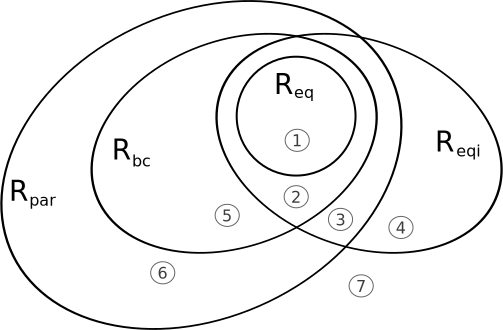
\includegraphics[width=300pt,height=241pt,keepaspectratio=true]
                    {containments.png}
  \end{center}
  \caption{ \label{fig:containments} Containment relationships for equivalence
    relations $R_{eq}$, $R_{eqi}$, $R_{bc}$, and $R_{par}$. The following are
    example elements in the sets at the specified locations: 1. (1100, 1100)
    2. (1010, 0101) 3. (1000, 0111) 4. (10000, 01111) 5. (1000, 0001) 6. (1000,
    1011) 7. (1000, 0000) }
\end{figure}


\section{Results}
\subsection{Reductions among equivalence relation}
\begin{theorem}$R_{par}\kr R_{bc}$\end{theorem}
\begin{proof}
\end{proof}
\begin{proof}
  Construct $M\in \FP$ on input $w\in\sigmastar$:
  \begin{algorithm}[h]
    \For{$i=1$ \KwTo $|w|-1$}{
      \If{$w_i=1$}{
        \For{$j=i+1$ \KwTo $|w|$}{
          \If{$w_j=1$}{
            write 0 to both $w_i$ and $w_j$\;
            break\;
          }
        }
      }
    }
  \end{algorithm}\\
  Notice that this is the machine which finds pairs of ones and writes zeros in
  their place, one pair at a time.

  Suppose $(x, y)\in R_{par}$, so either $x$ and $y$ both have even parity or
  $x$ and $y$ both have odd parity.
  
  If $x$ and $y$ both have even parity, $x$ contains $2k$ ones and $y$ contains
  $2l$ ones, for some $k,l\in\mathbb{N}$. $M(x)$ and $M(y)$ both output the
  string $0^{|x|}$, and since both $M(x)$ and $M(y)$ have a bitcount of zero,
  $(M(x), M(y))\in R_{bc}$.

  If $x$ and $y$ both have odd parity, $x$ contains $2k+1$ ones and $y$
  contains $2l+1$ ones, for some $k,l\in\mathbb{N}$. $M(x)$ and $M(y)$ both
  output a string containing a single one, so both $M(x)$ and $M(y)$ have a
  bitcount of one, $(M(x), M(y))\in R_{bc}$.

  Suppose $(x, y)\notin R_{par}$, so without loss of generality, $x$ has even
  parity and $y$ has odd parity. Then $x$ contains $2k$ ones and $y$ contains
  $2l+1$ ones, for some $k,l\in\mathbb{N}$. Thus $M(x)$ outputs the string
  $0^{|x|}$ and $M(y)$ outputs the string containing a single one. Since the
  bitcount of $M(x)$ is zero and the bitcount of $M(y)$ is one,
  $(M(x), M(y))\notin R_{bc}$.

  Therefore $(x, y)\in R_{par} \iff (M(x), M(y))\in R_{bc}$, so
  $R_{par} \kr R_{bc}$.
\end{proof}

\begin{theorem}$R_{bc}\kr R_{eq}$\end{theorem}
\begin{proof}
  Construct $M\in \FP$ on input $w\in\sigmastar$ which sorts the bits of $w$
  using an efficient (polynomial-time) sorting algorithm.

  Notice that if $|w|=n$ and $w$ contains $k$ ones, this machine outputs
  the string which can be described by the regular expression $0^{n-k}1^k$.

  Suppose $(x, y)\in R_{bc}$, so $x$ and $y$ have the same number of ones, say
  $k$. Thus $M(x)=M(y)=0^{n-k}1^k$, so $(M(x), M(y))\in R_{eq}$.
  
  Suppose $(x, y)\notin R_{bc}$, so $x$ and $y$ have a different number of
  ones. Suppose $x$ has $k$ ones and $y$ has $l$ ones, for some
  $k,l\in\mathbb{N}$. Assume without loss of generality that $k>l$. Then
  $M(x)=0^{n-k}1^{k}$ and $M(y)=0^{n-l}1^{l}$, so $M(x)\neq M(y)$. Thus
  $(M(x), M(y))\notin R_{eq}$.

  Therefore $(x, y)\in R_{bc} \iff (M(x), M(y))\in R_{eq}$, so $R_{bc}\kr
  R_{eq}$.
\end{proof}


\subsection{Reductions from equivalence relations to graph isomorphism}
%% \begin{lemma}\label{lem:gi_kr_dirgi}$GI\kr DirGI$\end{lemma}
%% \begin{proof}
%%   Construct machine $M\in\FP$ on input $G=(V,E)$:\\
%%   \begin{algorithm}[H]
%%     $V'\gets V$\;
%%     $E'\gets\{\}$\;
%%     \ForEach{$(u, v)\in E$}{
%%       add directed edges $(u, v)$ and $(v, u)$ to $E'$
%%     }
%%     \Return{$G'=(V', E')$}
%%   \end{algorithm}
%%   Notice that this machine constructs the graph with all undirected edges of
%%   the input graph replaced with two complementary directed edges incident to
%%   both vertices.

%%   %% TODO complete this proof
%% \end{proof}

%% \begin{lemma}\label{lem:dirgi_kr_gi}$DirGI\kr GI$\end{lemma}
%% \begin{proof}
%%   %% TODO complete this proof
%% \end{proof}

%% TODO are these kernel reductions? they must be...

%% There are other languages that are polynomial time kernel equivalent to
%% graph isomorphism, including but not limited to finite automata equivalence,
%% context-free grammar equivalence, multigraph isomorphism, hypergraph
%% isomorphism, etc.

\begin{theorem}\label{thm:rpar_gi}$R_{par}\kr GI$\end{theorem}
\begin{proof}
  Construct $M\in \FP$ on input $w\in\sigmastar$:\\
  \begin{algorithm}[H]
    $V_w\gets\{v_p, v_o\}$\;
    $E_w\gets\{\}$ \tcp{undirected edges}\;
    \For{$i=1$ \KwTo $|w|$}{
      \If{$w_i=1$}{
        \eIf{$(v_o, v_p)\in E_w$}{add undirected edge $(v_o, v_p)$ to $E_w$\;}
            {remove $(v_o, v_p)$ from $E_w$\;}
      }
    }
    \Return $G_w=(V_w, E_w)$
  \end{algorithm}

  Suppose $(x, y)\in R_{par}$, so either $x$ and $y$ both have even parity or
  $x$ and $y$ both have odd parity. 

  If $x$ and $y$ both have even parity, $x$ contains $2k$ ones and $y$ contains
  $2l$ ones, for some $k,l\in\mathbb{N}$. Since $2k$ is even, machine $M$ on
  input $x$ adds then removes the edge $(v_o, v_p)$ to and from $E_x$ an equal
  number of times. Similarly for $M$ on input $y$. Therefore $M(x)$ outputs
  $G_x=(V_x, E_x)$, where $V_x=\{v_o, v_p\}$ and $E_x=\{\}$, and $M(y)$ outputs
  $G_y=(V_y, E_y)$, where $V_y=\{v_o, v_p\}$ and $E_y=\{\}$. Then $G_x$ is
  isomorphic to $G_y$ by the identity function, $I:V_x\to V_y$, defined by
  $I(v)=v, \forall v\in V_x$.

  If $x$ and $y$ both have odd parity, $x$ contains $2k+1$ ones and $y$
  contains $2l+1$ ones, for some $k,l\in\mathbb{N}$. Since $2k+1$ is odd,
  machine $M$ on input $x$ adds edge $(v_o, v_p)$ to $E_x$ one more time than
  it removes the edge. Similarly for $M$ on input $y$. Therefore $M(x)$ outputs
  $G_x=(V_x, E_x)$, where $V_x=\{v_o, v_p\}$ and $E_x=\{(v_o, v_p)\}$, and
  $M(y)$ outputs $G_y=(V_y, E_y)$, where $V_y=\{v_o, v_p\}$ and $E_y=\{(v_o,
  v_p)\}$. Then $G_x$ is isomorphic to $G_y$ by the identity function,
  $I:V_x\to V_y$, defined by $I(v)=v, \forall v\in V_x$.

  Suppose $(x, y)\notin R_{par}$, so without loss of generality, $x$ has even
  parity and $y$ has odd parity. Then $x$ contains $2k$ ones and $y$ contains
  $2l+1$ ones, for some $k,l\in\mathbb{N}$. Since $2k$ is even, machine $M$ on
  input $x$ adds then removes the edge $(v_o, v_p)$ to and from $E_x$ an equal
  number of times. Since $2l+1$ is odd, machine $M$ on input $y$ adds edge
  $(v_o, v_p)$ to $E_y$ one more time than it removes the edge. Therefore
  $M(x)$ outputs $G_x=(V_x, E_x)$, where $V_x=\{v_o, v_p\}$ and $E_x=\{\}$, and
  $M(y)$ outputs $G_y=(V_y, E_y)$, where $V_y=\{v_o, v_p\}$ and $E_y=\{(v_o,
  v_p)\}$. Since $(v_o, v_p)\in E_y$ but $(v_o, v_p)\notin E_x$, so no
  bijection exists between $V_x$ and $V_y$ which preserves edges. Therefore,
  $G_x$ is not isomorphic to $G_y$ so $(M(x), M(y))\notin GI$.

  Therefore $(x, y)\in R_{par} \iff (M(x), M(y)) \in GI$, so $R_{par} \kr GI$.
\end{proof}

\begin{theorem}\label{thm:rbc_gi}$R_{bc}\kr GI$\end{theorem}
\begin{proof}
  Construct $M\in \FP$ on input $w \in \sigmastar$:\\
  \begin{algorithm}[H]
    $V_w\gets\{v_1, v_2, \ldots, v_{|w|}, v_{zero}, v_{one,0}, v_{one,1},
    v_{one,2}\}$\;
    $E_w\gets\{(v_{one,0}, v_{one,1}), (v_{one,1}, v_{one,2}), (v_{one,2},
    v_{one,0})\}$\tcp{undirected edges}\; 
    \For{$i=1$ \KwTo $|w|$}{
      \eIf{$w_i=1$}{
        add undirected edge $(v_i, v_{one,0})$ to $E_w$\;
      }{
        add undirected edge $(v_i, v_{zero})$ to $E_w$\;
      }
    }
    \Return{$G_w=(V_w, E_w)$}
  \end{algorithm}
  
  Suppose $(x, y)\in R_{bc}$, so $x$ and $y$ have the same number of ones, say
  $k\in\mathbb{N}$. Assume $|x|=|y|=n$, so both $x$ and $y$ have $n-k$
  zeros. Define $E_{w,1}=\{(v_i, v_{one,0})|i\in\{1,2,\ldots,n\}, w_i = 1\}$
  and $E_{w,0}=\{(v_i, v_{zero})|i\in\{1,2,\ldots,n\}, w_i = 0\}$, so $E_x =
  E_{x,1}\cup E_{x,0}$ and $E_y = E_{y,1} \cup E_{y,0}$ by construction. Define
  $V_{w,b}=\{v_i|w_i=b\}$, so $V_x=V_{x,1} \cup V_{x,0}$ and $V_y=V_{y,1} \cup
  V_{y,0}$. Note that $|V_{x,1}|=|V_{y,1}|=k$ and
  $|V_{x,0}|=|V_{y,0}|=n-k$. Since $|V_{x,1}|=|V_{y,1}|=k$, there exists a
  bijection between them, call it $\phi_1:V_{x,1}\to V_{y,1}$. Similarly, since
  $|V_{x,0}|=|V_{y,0}|=k$, there exists a bijection between them, call it
  $\phi_0:V_{x,0}\to V_{y,0}$. Define $\phi:V_x\to V_y$ by
  \begin{displaymath}
    \phi(v) = 
    \begin{cases}
      \phi_0(v) & \plain{if} v = v_i \plain{and} x_i = 1, \plain{for some}
      i\in\{1,\ldots,n\}\\ 
      \phi_1(v) & \plain{if} v = v_i \plain{and} x_i = 0, \plain{for some}
      i\in\{1,\ldots,n\}\\ 
      v & \plain{if} v \in \{v_{zero}, v_{one,0}, v_{one,1}, v_{one,2}\}
    \end{cases}
  \end{displaymath}
  for all $v\in V_x$. Notice that each $v_i$ ``corresponds'' to a
  single $x_i$, because each $x_i$ can be either a one or a zero,
  exclusively.

  Since the only edges in $E_x$ are the edges $(v_i, v_{one,0})$ when $x_i=1$
  and $(v_i, v_{zero})$ when $x_i=0$, then $(v_i, v_{one,0})\in E_x \iff
  (\phi(v_i), \phi(v_{one,0}))=(\phi_1(v_i), v_{one,0})\in E_y$, and $(v_i,
  v_{zero})\in E_x \iff (\phi(v_i), \phi(v_{zero})) = (\phi_0(v_i),
  v_{zero})\in E_y$. Therefore $\phi$ describes a graph isomorphism, so $G_1$
  is isomorphic to $G_2$.
  
  Suppose $(x, y)\notin R_{bc}$, so $x$ and $y$ have a different number of
  ones. Let $k$ be the number of ones in $x$, and $l$ be the number of ones in
  $y$, with $k\neq l$. Suppose without loss of generality that $k>l$. Define
  $E_{w,0}$ and $E_{w,1}$ as above. Now $|E_{x,1}|=k$ and $|E_{y,1}|=l$. Since
  $k>l$, $E_{x,1}$ has at least one more edge adjacent to the triangle created
  by the vertices $\{v_{one,0},v_{one,1},v_{one,2}\}$ than does $E_{y,1}$. Thus
  no possible bijection exists between $V_x$ and $V_y$ which preserves all
  edges. Thus $G_x$ is not isomorphic to $G_y$, so $(M(x), M(y))\notin GI$.

  Therefore $(x, y)\in R_{bc} \iff (M(x), M(y))\in GI$, so $R_{bc}\kr GI$.
\end{proof}

Unlike the reductions from $R_{par}$ and $R_{bc}$ to $GI$, in the reductions
from $R_{eq}$ and $R_{eqi}$ to $GI$ the order of bits in each string $x$ and
$y$ is significant. Therefore, we can use the following lemma to reduce these
equivalence relation problems to the directed form of the graph isomorphism
problem.

\begin{lemma}\label{lem:gi_ke_dirgi}$GI\kequiv DirGI$\end{lemma}
\begin{proof}
  %% TODO complete this proof
  %% provide simply a reference? see the graph isomorphism book
\end{proof}

From Lemma \ref{lem:gi_ke_dirgi}, we can use a kernel reduction to directed
graph isomorphism to show that a language kernel reduces to (undirected) graph
isomorphism, as in the following two theorems.

\begin{theorem}\label{thm:req_kr_dirgi}$R_{eq} \kr DirGI$\end{theorem}
\begin{proof}
  Construct machine $M\in\FP$ on input $w\in\sigmastar$:\\
  \begin{algorithm}[H]
    $V_w\gets\{v_1, v_2, \ldots, v_{|w|}\}$\; 
    $E_w\gets\{(v_1, v_2), (v_2, v_3), \ldots, (v_{|w|-1},
    v_{|w|})\}$\tcp*[f]{directed edges}\;
    \For{$i=1$ \KwTo $|w|$}{
      \If{$w_i=1$}{
        add vertex $v'_i$ to $V_w$\;
        add directed edge $(v_i, v'_i)$ to $E_w$\;
      }
    }
    \Return{$G_w=(V_w, E_w)$}
  \end{algorithm}
  Notice that this machine constructs a ``spine'' of vertices, with an extra
  vertex $v'_i$ and directed edge $(v_i, v'_i)$ adjacent to the spine whenever
  $w_i$ is a one, $\forall i\in\{1,2,\ldots,|w|\}$.

  Suppose $(x, y)\in R_{eq}$, so $x=y$. Then $M(x)$ and $M(y)$ produce the same
  graph, so $G_x$ is isomorphic to $G_y$ by the identity mapping. Therefore
  $(M(x), M(y))\in DirGI$.
  
  %% TODO is this sufficient proof?

  Suppose $(x, y)\notin R_{eq}$, so $x\neq y$. Suppose $|x|=|y|=n$. Run $M$ on
  input $x$ to yield $G_x=(V_x, E_x)$, and run $M$ on input $y$ to yield
  $G_y=(V_y, E_y)$. Since the graphs are directed, the ``spine'' created by the
  vertices $\{v_1, v_2, \ldots, v_n\}$ and the edges $\{(v_1, v_2), (v_2, v_3),
  \ldots, (v_{n-1}, v_n)\}$ must correspond in both $G_x$ and $G_y$. Let $i$ be
  the index of the first bit at which $x$ and $y$ differ. Suppose without loss
  of generality that $x_i=1$ and $y_i=0$. Then $v'_i\in V_x$ and $(v_i,
  v'_i)\in E_x$, but $v'_i\notin V_y$ so $(v_i, v'_i)\notin E_y$. Assume with
  the intention of producing a contradiction that a bijection exists between
  $V_x$ and $V_y$ which satisfies the conditions for a graph isomorphism. Since
  vertices along the ``spine'' of the $V_x$ must map to vertices along the
  ``spine'' of $V_y$, and specifically $v_i$ in $V_x$ must map to $v_i$ in
  $V_y$, $(v_i, v'_i)\in E_x$ implies $(v_i, v'_i)\in E_y$. But $(v_i,
  v'_i)\notin E_y$ because $y_i=0$. This is a contradiction. Therefore no such
  mapping exists, so $G_x$ is not isomorphic to $G_y$, and hence $(M(x),
  M(y))\notin DirGI$.

  Therefore $(x, y)\in R_{eq} \iff (M(x), M(y))\in DirGI$, so $R_{eq}\kr
  DirGI$.
\end{proof}

\begin{corollary}$R_{eq}\kr GI$\end{corollary}
\begin{proof}Follows directly from Theorem \ref{thm:req_kr_dirgi} and Lemma
  \ref{lem:gi_ke_dirgi}.\end{proof}

\begin{theorem}\label{thm:reqi_kr_dirgi}$R_{eqi}\kr DirGI$\end{theorem}
\begin{proof}
  Construct machine $M\in \FP$ on input $w\in\sigmastar$:\\
  \begin{algorithm}[H]
    $V_w\gets\{v_1, v_2, \ldots, v_{|w|}, v_{zero}, v_{one}\}$\;
    $E_w\gets\{(v_1, v_2), (v_2, v_3), \ldots, (v_{|w|-1},
    v_{|w|})\}$\tcp*[f]{directed edges}\;
    \For{$i=1$ \KwTo $|w|$}{
      \eIf{$w_i=1$}{
        add directed edge $(v_i, v_{one})$ to $E_w$
      }{
        add directed edge $(v_i, v_{zero})$ to $E_w$
      }
    }
    \Return{$G_w=(V_w, E_w)$}
  \end{algorithm}
  Notice that this machine, as in the machine in the proof of Theorem
  \ref{thm:req_kr_dirgi}, creates a ``spine'' representing each bit of word
  $w$.

  Suppose $(x, y)\in R_{eqi}$, so either $x=y$ or $x=\bar{y}$.

  In the case that $x=y$, $M(x)$ and $M(y)$ output exactly the same graph, so
  $G_x$ is isomorphic to $G_y$, and hence $(M(x), M(y))\in DirGI$.

  In the case that $x=\bar{y}$, define $\phi:V_x\to V_y$ by
  \begin{displaymath}
    \phi(v)=
    \begin{cases}
      v & \plain{if} v = v_i, \plain{for some} i\in\{1, 2, \ldots, |x|\}\\
      v_{zero} & \plain{if} v = v_{one}\\
      v_{one} & \plain{if} v = v_{zero}
    \end{cases}
  \end{displaymath}
  for all $v\in V_x$. Notice that $\phi$ maps each $v_i\in V_x$ to the
  corresponding $v_i\in V_y$, and maps $v_{zero}\in V_x$ to $v_{one}\in V_y$
  and $v_{one}\in V_x$ to $v_{zero}\in V_y$. Then $\forall
  i\in\{1,2,\ldots,|x|\}$, $x_i=0 \iff y=1$, so $(v_i, v_{zero})\in E_x \iff
  (\phi(v_i), \phi(v_{zero})) = (v_i, v_{one})\in E_y$. Similarly, $x_i=1 \iff
  y=0$, so $(v_i, v_{one})\in E_x \iff (\phi(v_i), \phi(v_{one}))\in E_y \iff
  (v_i, v_{zero})\in E_y$. The rest of the edges in $E_x$ map directly to the
  corresponding edges in $E_y$ by $(v_{i-1}, v_i) \mapsto (\phi(v_{i-1}),
  \phi(v_i))=(v_{i-1}, v_i)$, $\forall i\in\{2,3,\ldots,|x|\}$. Therefore,
  $\phi$ describes an isomorphism between $G_x$ and $G_y$, so $(M(x), M(y))\in
  DirGI$.

  Suppose $(x, y)\notin R_{eqi}$, so $x\neq y$ and $x\neq\bar{y}$. Thus
  $\exists i,j\in\{1,2,\ldots,|x|\}, i\neq j,$ such that $x_i=y_i\land x_j\neq
  y_j$. Suppose without loss of generality that $x_i=y_i=0$ and $0=x_j\neq
  y_j=1$. Now $x_i=y_i=0$ implies $(v_i, v_{zero})\in E_x$ and $(v_i,
  v_{zero})\in E_y$. Also, $x_j=0$ implies $(v_j, v_{zero})\in E_x$ and $y_j=1$
  implies $(v_j, v_{one})\in E_y$. Assume, with the goal of producing a
  contradiction, that there exists a bijection, $\phi:V_x\to V_y$ such that
  $(u,v)\in E_x\iff(\phi(u),\phi(v))\in E_y$, $\forall u,v\in V_x$. Since
  $\phi$ must map vertices on the ``spine'' of $G_x$ to corresponding vertices
  in $G_y$, and since $(v_i, v_{zero})\in E_x$, then $(\phi(v_i),
  \phi(v_{zero}))=(v_i, \phi(v_{zero}))$ must be in $E_y$. The only edge of
  this form in $E_y$ is $(v_i, v_{zero})$ so $\phi(v_{zero})=v_{zero}$. Since
  $(v_j, v_{zero})\in E_x$, $(\phi(v_j), \phi(v_{zero}))=(v_j, v_{zero})\in
  E_y$. But the only edge in $E_y$ with source vertex $v_j$ is, by
  construction, $(v_j, v_{one})$. This is a contradiction. Hence no such
  bijection exists, so $G_x$ is not isomorphic to $G_y$, and $(M(x),
  M(y))\notin DirGI$.

  Therefore $(x, y)\in R_{eqi} \iff (M(x), M(y))\in DirGI$, so $R_{eqi}\kr
  DirGI$.
\end{proof}

\begin{corollary}$R_{eqi}\kr GI$\end{corollary}
\begin{proof}Follows directly from Theorem \ref{thm:reqi_kr_dirgi} and Lemma
  \ref{lem:gi_ke_dirgi}.\end{proof}

\begin{theorem}\label{thm:ra_kr_dirgi}$\forall a\in\sigmastar R_a \kr DirGI$
\end{theorem}
\begin{proof}
  Let $a\in\sigmastar$. Construct machine $M\in\FP$ on input $w\in\sigmastar$
  (let $n=|w|$):\\
  \begin{algorithm}[H]
    $U_w\gets\{v_1, v_2, \ldots, v_n\}$\;
    $U'_w\gets\{v'_1, v'_2, \ldots, v'_n\}$\;
    $F_w\gets\{(v_1, v_2), (v_2, v_3), \ldots, (v_{n-1},
    v_n)\}$\tcp*[f]{directed edges}\;
    $F'_w\gets\{(v'_1, v'_2), (v'_2, v'_3), \ldots, (v'_{n-1},
    v'_n)\}$\tcp*[f]{directed edges}\;
    \For{$i=1$ \KwTo $n$}{
      \If{$w_i=1$}{
	add vertex $u_i$ to $U_w$\;
	add directed edge $(v_i, u_i)$ to $F_w$\;
      }
      \If{$w_i\oplus a_i=1$}{
	add vertex $u'_i$ to $U'_w$\;
	add directed edge $(v'_i, u'_i)$ to $F'_w$\;
      }
    }
    $V_w\gets U_w\cup U'_w$\;
    $E_w\gets F_w\cup F'_w$\;
    \Return{$G_w=(V_w, E_w)$}
  \end{algorithm}
  Notice that for each input string $w$, this machine produces a graph which is
  the disjoint union of two distinct graphs, one representing the bits of $w$
  and the other representing the bits of $w\oplus a$.
  
  Suppose $(x,y)\in R_a$, so either $x=y$ or $x\oplus y=a$.
  
  In the case that $x=y$, $M(x)$ and $M(y)$ output exactly the same graph, so
  $G_x$ is isomorphic to $G_y$, and hence $(M(x), M(y))\in DirGI$.
  
  Consider the case in which $x\neq y$, but $x\oplus y=a$. Define $\phi:V_x\to
  V_y$ by
  \begin{displaymath}
    \phi(v)=
    \begin{cases}
      v'_i & \plain{if} v=v_i \plain{for some} i\in\{1, 2, \ldots, n\}\\
      v_i & \plain{if} v=v'_i \plain{for some} i\in\{1, 2, \ldots, n\}\\
      u'_i & \plain{if} v=u_i \plain{for some} i\in\{1, 2, \ldots, n\}\\
      u_i & \plain{if} v=u'_i \plain{for some} i\in\{1, 2, \ldots, n\}\\
    \end{cases}
  \end{displaymath}
  If no $u_i$ exists or no $u'_i$ exists for some $i\in\{1, 2, \ldots, n\}$
  then we don't define $\phi$ for those values not in the domain. $\phi$ maps
  each $v_i\in V_x$ to $v'_i\in V_y$, so $(v_i, v_{i+1})\in E_x \iff
  (\phi(v_i), \phi(v_{i+1}))=(v'_i, v'_{i+1})\in E_y, \forall i\in\{1, 2,
  \ldots, n-1\}$, and $\phi$ maps each $v'_i\in V_x$ to $v_i\in V_y$, so
  $(v'_i, v'_{i+1})\in E_x \iff (\phi(v'_i), \phi(v'_{i+1}))=(v_i, v_{i+1})\in
  E_y, \forall i\in\{1, 2, \ldots, n-1\}$.

  Now for each $i\in\{1, 2, \ldots, n\}$ for which $u_i$ exists and is in
  $V_x$, $(v_i, u_i)\in E_x$ by construction. This occurs if and only if
  $x_i=1$, and since by hypothesis $x\oplus y=a \iff y=x\oplus a$,
  $y_i=x_i\oplus a_i$. In the case that $a_i=0$, then $y_i=x_i\oplus a_i=
  1\oplus 0=1$. Since $y_i=1$ and $y_i\oplus a_i=1\oplus 0=1$, $M(y)$ produces
  graph $G_y$ containing vertex $u'_i\in V_y$ and directed edge $(v'_i,
  u'_i)\in E_y$. Now $\phi(u_i)=u'_i$ is well-defined, and $(v_i, u_i)\in
  E_x\iff (\phi(v_i), \phi(u_i))=(v'_i, u'_i)\in E_y$. In the case that
  $a_i=1$, then $y_i=x_i\oplus a_i=1\oplus1=0$. Since $y_i=0$ and $y_i\oplus
  a_i=0\oplus 1=1$, $M(y)$ produces graph $G_y$ containing vertex $u'_i\in V_y$
  and directed edge $(v'_i, u'_i)\in E_y$. Now $\phi(u_i)=u'_i$ is
  well-defined, and $(v_i, u_i)\in E_x\iff (\phi(v_i), \phi(u_i))=(v'_i,
  u'_i)\in E_y$.

  Now for each $i\in\{1, 2, \ldots, n\}$ for which $u'_i$ exists and is in
  $V_x$, $(v'_i, u'_i)\in E_x$ by construction. This occurs if and only if
  $x_i\oplus a_i=1$, and since by hypothesis $x\oplus y=a \iff y=x\oplus a$,
  then $y_i=x_i\oplus a_i=1$. Since $y_i=1$, $M(y)$ produces graph $G_y$
  containing vertex $u_i\in V_y$ and directed edge $(v_i, u_i)\in E_y$. Now
  $\phi(u'_i)=u_i$ is well-defined, and $(v'_i, u'_i)\in E_x\iff (\phi(v'_i),
  \phi(u'_i))=(v_i, u_i)\in E_y$. Therefore $\phi$ describes an isomorphism
  between graphs $G_x$ and $G_y$, so $(M(x),M(y))\in DirGI$.

  Suppose $(x, y)\notin R_a$, so $x\neq y$ and $x\oplus y\neq a$. Thus $\exists
  i,j\in\{1, 2, \ldots, n\}: x_i\neq y_i$ and $x_j\oplus y_j\neq a_j$ (with the
  possibility that $i=j$). Because $M(x)$ and $M(y)$ both produce graphs which
  are the disjoint union of two distinct subgraphs, $(U_x, F_x)$ and $(U'_x,
  F'_x)$ in $G_x$ and $(U_y, F_y)$ and $(U'_y, F'_y)$ in $G_y$, if the graphs
  $G_x$ and $G_y$ were isomorphic, the bijection between them must either map
  vertices of $U_x$ to $U_y$ and $U'_x$ to $U'_y$ or map vertices of $U_x$ to
  $U'_y$ and $U'_x$ to $U_y$. The only possible bijections must map either
  $v_i\in U_x$ to $v_i\in U_y$ and $v'_i\in U'_x$ to $v'_i\in U'_y$ or $v_i\in
  U_x$ to $v'_i\in U'_y$ and $v'_i\in U'_x$ and $v_i\in U_y$, $\forall i\in\{1,
  2, \ldots, n\}$, because of the chain of directed edges between each vertex
  of adjacent index.

  Assume without loss of generality that $x_i=1$ and $y_i=0$, which implies
  $(v_i, u_i)\in F_x$ but $(v_i, u_i)\notin F_y$. Now $\phi$ cannot map $v_i\in
  U_x$ to $v_i\in U_y$ and $v'_i\in U'_x$ to $v'_i\in U'_y$ because $(v_i,
  u_i)\in F_x$ but $(v_i, u_i)\notin F_y$. 

  Assume $\phi$ describes a graph isomorphism which maps $v_j\in U_x$ to
  $v'_j\in U'_y$ and $v'_j\in U'_x$ to $v_j\in U_y$. In the case that $x_j=0$,
  $y_j=0$ and $a_j=1$, then $y_j\oplus a_j=1$, so $(v_j, u_j)\notin F_x$ but
  $(v'_j, u'_j)\in F'_y$. This is a contradiction with the assumption that
  $\phi$ describes a graph isomorphism. In the case that $x_j=1$, $y_j=1$ and
  $a_j=1$, then $y_j\oplus a_j=0$, so $(v_j, u_j)\in F_x$ but $(v'_j,
  u'_j)\notin F'_y$. This is a contradiction. In the case that $x_j=0$,
  $y_j=1$, and $a_j=0$, then $y_j\oplus a_j=1$, so $(v_j, u_j)\notin F_x$ but
  $(v'_j, u'_j)\in F'_y$. This is a contradiction. In the case that $x_j=1$,
  $y_j=0$, and $a_j=0$, then $y_j\oplus a_j=0$, so $(v_j, u_j)\in F_x$ but
  $(v'_j, u'_j)\notin F'_y$. This is a contradiction. Therefore no such
  bijection $\phi$ exists. Therefore $G_x$ is not isomorphic to $G_y$, thus
  $(M(x), M(y))\notin DirGI$.

  Therefore $(x, y)\in R_a\iff (M(x), M(y))\in DirGI$, so $R_a\kr DirGI$.
\end{proof}

\begin{corollary}$R_a\kr GI$\end{corollary}
\begin{proof}Follows directly from Theorem \ref{thm:ra_kr_dirgi} and Lemma
  \ref{lem:gi_ke_dirgi}.\end{proof}


\subsection{Completeness}
\begin{definition}
  \hangindent=1.2in
  $R_{KC}=\{((G_1, k_1), (G_2, k_2))| k_1=k_2 \plain{and} (G_1\cong G_2
  \plain{or}\\ (G_1 \plain{has a clique of size} k_1 \plain{and} G_2 \plain{has
  a clique of size} k_2))\}$
\end{definition}

\begin{theorem}$R_{KC}$ is an equivalence relation.\end{theorem}
\begin{proof}To show that $R_{KC}$ is an equivalence relation, we must show
  that it is reflexive, symmetric, and transitive.

  Since $G$ is isomorphic to $G$ for all graphs $G$, $((G,k),(G,k))\in R_{KC}$,
  for all $k\in\mathbb{N}$, so $R_{KC}$ is reflexive.

  To show that $R_{KC}$ is symmetric, suppose $((G_1, k_1), (G_2, k_2))\in
  R_{KC}$. In the case that $G_1$ is isomorphic to $G_2$, then $G_2$ is
  isomorphic to $G_1$ because the isomorphism relation is symmetric, so
  $((G_2,k_2),(G_1,k_1))\in R_{KC}$. In the case that $G_1$ has a clique of
  size $k_1$ and $G_2$ has a clique of size $k_2$ and $k_1=k_2$, then
  $((G_2,k_2),(G_1,k_1))\in R_{KC}$ because the logical conjunction operation
  is commutative over propositions.

  To show that $R_{KC}$ is transitive, suppose $((G_1, k_1), (G_2, k_2))\in
  R_{KC}$ and $((G_2, k_2), (G_3, k_3))\in R_{KC}$. Since $k_1=k_2$ and
  $k_2=k_3$, then $k_1=k_3$ by the transitivity of the equality relation. There
  are four possible cases for the remaining properties.

  In the case that $G_1$ is isomorphic to $G_2$ and $G_2$ is isomorphic to
  $G_3$, then $G_1$ is isomorphic to $G_3$ so $((G_1, k_1), (G_3, k_3))\in
  R_{KC}$.

  In the case that $G_1$ is isomorphic to $G_2$, $G_2$ has a clique of size
  $k_2$, $G_3$ has a clique of size $k_3$, then $G_1$ has a clique of size
  $k_2=k_1$, so $((G_1, k_1), (G_3, k_3))\in R_{KC}$.

  In the case that $G_1$ has a clique of size $k_1$, $G_2$ has a clique of size
  $k_2$, and $G_2$ is isomorphic to $G_3$, then $G_3$ has a clique
  of size $k_2=k_3$, so $((G_1, k_1), (G_3, k_3))\in R_{KC}$.

  In the case that $G_1$ has a clique of size $k_1$, $G_2$ has a clique of size
  $k_2$, and $G_3$ has a clique of size $k_3$, then $((G_1, k_1), (G_3,
  k_3))\in R_{KC}$.

  Therefore $R_{KC}$ is reflexive, symmetric, and transitive, hence it is an
  equivalence relation.
\end{proof}

\begin{definition}$CLIQUE=\{(G,k)|G \plain{has a clique of size}
  k\}$\end{definition}

\begin{lemma}$CLIQUE$ is \NP-complete.\end{lemma}
\begin{proof}
  The proof is a polynomial time reduction from $3SAT$, which is \NP-complete.
\end{proof}

%% TODO rewrite algorithms using \KwIn and \KwOut
\begin{lemma}\label{lem:rkc_np}$R_{KC}\in\NP$\end{lemma}
\begin{proof}
  Since $GI\in\NP$, it has a deterministic polynomial time verifier, $M_1$,
  which accepts on input $(G_1, G_2, c)$, where $c$ is the isomorphism from
  vertices of $G_1$ to vertices of $G_2$.

  Since $CLIQUE\in\NP$, it has a deterministic polynomial time verifier, $M_2$,
  which accepts on input $(G, k, c)$, where $c$ is the set of vertices in $G$
  which comprise a clique of size $k$.

  To show that $R_{KC}\in\NP$, we construct a deterministic polynomial time
  verifier $M$ for $R_{KC}$. On input $(((G_1, k_1), (G_2, k_2)), c)$:\\
  \begin{algorithm}[H]
    If $k_1\neq k_2$, \REJECT\;
    \If{$c$ \textnormal{is the encoding of a mapping}}{
      Run $M_1$ on input $(G_1, G_2, c)$\;
      If $M_1$ accepts, \ACCEPT; otherwise \REJECT\;
    }
    \If{$c=(c_1, c_2)$ \textnormal{is the encoding of two cliques}}{
      Run $M_2$ on input $(G_1, k_1, c_1)$\;
      Run $M_2$ on input $(G_2, k_2, c_2)$\;
      If $M_2$ accepts on both inputs, \ACCEPT; otherwise \REJECT\;
    }
  \end{algorithm}
  
  Machine $M$ is a verifier for $R_{KC}$, so $R_{KC}\in\NP$.
\end{proof}

\begin{corollary}\label{cor:rkc_npeq}$R_{KC}\in\NPEq$\end{corollary}
\begin{proof}
  Since $R_{KC}\in\NP$ by \autoref{lem:rkc_np} and $R_{KC}$ is an equivalence
  problem, then by \autoref{def:peq}, $R_{KC}\in\NPEq$.
\end{proof}

\begin{theorem}\label{thm:rkc_npc}$R_{KC}$ is \NP-complete.\end{theorem}
\begin{proof}
  Since $R_{KC}\in\NP$ by \autoref{lem:rkc_np}, we need only show that $R_{KC}$
  is \NP-hard. To do this, we construct a polynomial time many-one reduction
  from $CLIQUE$, which is \NP-complete, to $R_{KC}$.

  Construct machine $M\in\FP$ on input $(G, k)$ which outputs $((G, k), (K_k,
  k))$, where $K_k$ is the complete graph with $k$ vertices.

  Suppose $(G,k)\in CLIQUE$, so $G$ has a clique of size $k$. Then
  $M((G,k))=((G,k), (K_k, k))\in R_{KC}$, because $G$ has a clique of size
  $k$ by hypothesis and $K_k$ has a clique of size $k$ by construction,
  specifically, the set of all vertices in $K_k$.
  
  Suppose $(G,k)\notin CLIQUE$, so $G$ does not have a clique of size $k$ and
  $M((G,k))=((G,k), (K_k, k))$. If $G$ were isomorphic to $K_k$, then it would
  have a clique of size $k$, specifically the set of all its vertices, but this
  is a contradiction with the hypothesis so no such isomorphism
  exists. Although $K_k$ certainly has a clique of size $k$, specifically the
  set of all its vertices, $G$ does not have a clique of size $k$ by
  hypothesis, so $((G, k), (K_k, k))\notin R_{KC}$.
  
  Therefore $(G,k)\in CLIQUE\iff M((G,k))\in R_{KC}$, so $CLIQUE\mor R_{KC}$,
  and hence $R_{KC}$ is \NP-complete.
\end{proof}

\begin{theorem}$\NPC\cap\NPEq\neq\emptyset$\end{theorem}
\begin{proof}
  By \autoref{cor:rkc_npeq}, $R_{KC}\in\NPEq$, and by \autoref{thm:rkc_npc},
  $R_{KC}\in\NPC$, so $R_{KC}\in\NPEq\cap\NPC$.
\end{proof}

Since $R_{KC}$ is both in $\NPEq$ and \NP-complete, we want to show that it may
be a candidate for an \NPEq-complete, problem. In other words, is it true that
all equivalence problems in $\NPEq$ kernel reduce to $R_{KC}$? A handful of
equivalence problems in $\NPEq$ kernel reduce to graph isomorphism, and as the
following theorem shows, we can kernel reduce the graph isomorphism problem to
$R_{KC}$.

\begin{theorem}$GI\kr R_{KC}$\end{theorem}
\begin{proof}
  Construct machine $f\in\FP$ defined for all graphs $G=(V,E)$ by
  $f(G)=(G,|V|+1)$.

  Let $G_1=(V_1, E_1)$ and $G_2=(V_2, E_2)$, and suppose $(G_1, G_2)\in GI$, so
  $G_1$ is isomorphic to $G_2$. This implies $|V_1|=|V_2|$ and thus
  $|V_1|+1=|V_2|+1$. Now $f(G_1)=(G_1, |V_1|+1)$ and $f(G_2)=(G_2,
  |V_2|+1)$. Since $G_1$ is isomorphic to $G_2$ and $|V_1|+1=|V_2|+1$, then
  $((G_1, |V_1|+1),(G_2, |V_2|+1))=(f(G_1), f(G_2))\in R_{KC}$.
  
  Suppose $(G_1, G_2)\notin GI$, so $G_1$ is not isomorphic to $G_2$. Since
  $G_1$ cannot have a clique of size $|V_1|+1$, and further, since $G_2$ cannot
  have a clique of size $|V_2|+1$, then $((G_1, |V_1|+1), (G_2,
  |V_2|+1))=(f(G_1), f(G_2))\notin R_{KC}$.

  Therefore $(G_1, G_2)\in GI\iff (f(G_1), f(G_2))\in R_{KC}$, so $GI\kr
  R_{KC}$.
\end{proof}


%% TODO rewrite this section

Now the question is where does $\GIm$ live? There exist exotic problems which
are not equivalence problems, but which are polynomial-time many-one equivalent
to the graph isomorphism problem. For example, Kozen's M-tree clique problem,
the problem of recognizing a legitimate regular deck, and the problem of
recognizing a self-complementary graph are \emph{not} equivalence problems, but
they are indeed polynomial-time many-one equivalent to the graph isomorphism
problem. Since they are not equivalence relations, they certainly cannot be
kernel reduced to graph isomorphism, so $\GIker\subsetneq\GIm$.
%% TODO references

The next question is are there equivalence relations which many-one reduce to
graph isomorphism but which do not kernel reduce to graph isomorphism?
Informally, the question asks if there is some reduction relations such that
the reduction \emph{requires} information about both elements in each pair
(because a many-one reduction gets access to both elements $x$ and $y$ when
$(x,y)\in R$ whereas a kernel reduction gets access only to one at a time). In
fact, the problem of recognizing a self-complementary graph, when expressed as
an equivalence relation, may be a candidate for such a problem.

Examining most of the other problems in the class $\GIm$ reveals that nearly
all other (known) reductions can be expressed as kernel reductions. Many of the
techniques involve either edge replacement or composition of graphs, which can
both be performed on either graph without knowledge of the other. However, the
self-complementary graph problem, which is $SCGI=\{G|G \plain{is isomorphic to}
\bar{G}\}$, does not seem to have this property. Note that this set can be
alternately defined as an equivalence relation, $SCGI=\{(G_1,
G_2)|G_1=\bar{G_2} or \}$.


\section{References}
%\bibliography{references}

\end{document}
